% ROZDZIAŁ 26 — MIARA I WYMIAR HAUSDORFFA, TWIERDZENIE FROSTMANA
\chapter{Miara Hausdorffa i wymiar Hausdorffa}
\label{ch:hausdorff-26}

\providecommand{\atlasref}[2]{#2}


\section{Dlaczego miara Lebesgue'a nie wystarcza?}
Obraz ograniczonego przedziału przez odwzorowanie
Lipschitzowskie w $\mathbb R^2$ ma zerową miarę
$\lambda_2$, choć może mieć dodatnią długość.
Dla dowolnych krzywych ciągłych nie można tego
twierdzić (istnieją krzywe wypełniające kwadrat).
Zbiór Cantora ma zerową długość, ale posiada nietrywialną
strukturę w skali ułamkowego wymiaru. Celem tego
rozdziału jest skonstruowanie miar $\mathcal H^s$,
które mierzą zbiory odpowiednio do ich wymiaru, oraz
wyprowadzenie skutecznych kryteriów tego wymiaru.

\section{Konstrukcja miary Hausdorffa od podstaw}
\label{sec:hausdorff-konstrukcja-26}

\noindent\emph{Powiązanie tematyczne w Bibliotece matematycznej:} \atlasref{DG-11::def:miara-hausdorffa}{DG-11: miara Hausdorffa w geometrii różniczkowej}.


W tej sekcji przeprowadzimy całą konstrukcję, łącznie z
mierzalnością zbiorów borelowskich. Nie będziemy zakładać
twierdzenia, że metryczna miara zewnętrzna automatycznie
mierzy zbiory borelowskie: udowodnimy potrzebny fakt.
Wykorzystamy jedynie elementarne własności kresów,
przeliczalnych pokryć i odległości w przestrzeni metrycznej.

\begin{definicja}[Koszt pokrycia i miara Hausdorffa]
\label{def:hausdorff-measure-26}
Niech $(X,d)$ będzie przestrzenią metryczną, $s\geq0$
i $\delta>0$. Dla $U\subseteq X$ definiujemy
$\operatorname{diam}U:=\sup\{d(x,y):x,y\in U\}$,
przyjmując $\operatorname{diam}\varnothing=0$.
Ustalamy $c_s>0$, przy czym $c_0=1$.
Dla $s>0$ koszt zbioru to $h_s(U)=c_s(\operatorname{diam}U)^s$.
Dla $s=0$ przyjmujemy jawnie
$h_0(U)=0$ dla $U=\varnothing$ oraz $h_0(U)=1$
dla $U\neq\varnothing$, niezależnie od średnicy.
Definiujemy
\begin{equation}\label{eq:hausdorff-delta-26}
 \mathcal H^s_\delta(E)
 :=\inf\left\{\sum_{j=1}^\infty h_s(U_j):
 E\subseteq\bigcup_{j=1}^\infty U_j,\quad
 \operatorname{diam}U_j\leq\delta\right\}.
\end{equation}
Infimum pustej rodziny dopuszczalnych pokryć wynosi
$+\infty$; zbiór pusty ma koszt $0$ (pokrycie pustymi
zbiorami). \emph{Miarę Hausdorffa wymiaru $s$} określamy
wzorem
\begin{equation}\label{eq:hausdorff-26}
 \mathcal H^s(E):=\lim_{\delta\downarrow0}
 \mathcal H^s_\delta(E)
 =\sup_{\delta>0}\mathcal H^s_\delta(E).
\end{equation}
Jest to dobrze określona wartość z $[0,+\infty]$,
gdyż $0<\delta'<\delta$ pociąga za sobą
$\mathcal H^s_{\delta'}(E)\geq\mathcal H^s_\delta(E)$.
Dla $s>0$ popularna normalizacja to
$c_s=\omega_s2^{-s}$, gdzie
$\omega_s=\pi^{s/2}/\Gamma(1+s/2)$;
$\Gamma$ oznacza funkcję gamma Eulera, tj.
$\Gamma(t)=\int_{(0,+\infty)}u^{t-1}e^{-u}\,\mathrm d\lambda_1(u)$
dla $t>0$. Można jednak przyjąć $c_s=1$, nie zmieniając
własności mierzalności ani wymiaru Hausdorffa.
W przypadku $s=1$ standardowy wybór daje $c_1=1$.
\end{definicja}

Ważne jest rozdzielenie dwóch operacji: najpierw
wybieramy \emph{dowolne przeliczalne} pokrycie zbiorami
o średnicy co najwyżej $\delta$ i minimalizujemy koszt;
dopiero potem wymuszamy $\delta\downarrow0$.
Nie ograniczamy pokryć do kul ani do zbiorów mierzalnych.
W przestrzeni nieośrodkowej może nie istnieć przeliczalne
pokrycie danego $E$ o małych średnicach; wtedy
odpowiednia wartość jest po prostu nieskończona.

\begin{uwaga}[Miara a zawartość Hausdorffa]
Gdy w~\eqref{eq:hausdorff-delta-26} nie narzucamy
ograniczenia średnic, otrzymujemy \emph{zawartość
Hausdorffa} $\mathcal H^s_\infty(E)$. Sama zawartość
nie musi być addytywna nawet dla rozłącznych
zbiorów odległych od siebie: jedno duże pokrycie
może być tańsze od dwóch oddzielnych.
Dlatego warunek $\delta\downarrow0$ jest istotny.
\end{uwaga}

\begin{lemat}[Zewnętrzne własności kosztu pokryć]
\label{lem:hausdorff-outer-26}
Dla każdego $s\geq0$ i $\delta>0$ funkcja
$E\mapsto\mathcal H^s_\delta(E)$ spełnia:
$\mathcal H^s_\delta(\varnothing)=0$,
monotoniczność i przeliczalną podaddytywność.
To samo dotyczy funkcji $E\mapsto\mathcal H^s(E)$.
\end{lemat}
\begin{proof}
Pusta rodzina punktów nie wymaga żadnego pokrycia,
a pokrycie złożone ze zbiorów pustych ma koszt zero.
Jeśli $A\subseteq B$, każde pokrycie $B$ pokrywa $A$,
więc infimum dla $A$ nie przekracza infimum dla $B$.

Niech $E\subseteq\bigcup_{k\ge1}E_k$. Jeśli suma
$\sum_k\mathcal H^s_\delta(E_k)$ jest nieskończona,
nierówność podaddytywności jest automatyczna.
W przeciwnym razie wszystkie składniki są skończone.
Dla $\varepsilon>0$ i każdego $k$ wybieramy dopuszczalne
pokrycie $(U_{kj})_{j\ge1}$ zbioru $E_k$ o koszcie
nieprzekraczającym
$\mathcal H^s_\delta(E_k)+\varepsilon2^{-k}$.
Rodzina wszystkich $U_{kj}$ jest przeliczalna,
ma średnice co najwyżej $\delta$ i pokrywa $E$.
W konsekwencji
$\mathcal H^s_\delta(E)\leq
\sum_k\mathcal H^s_\delta(E_k)+\varepsilon$.
Przechodząc $\varepsilon\downarrow0$, otrzymujemy
podaddytywność na ustalonej skali.

Przy przejściu do granicy \emph{nie zamieniamy}
supremum z nieskończoną sumą. Dla każdego $\delta$
z poprzedniej nierówności i z definicji supremum mamy
$\mathcal H^s_\delta(E)\leq
\sum_k\mathcal H^s_\delta(E_k)
\leq\sum_k\mathcal H^s(E_k)$.
Wzięcie supremum po $\delta>0$ kończy dowód.
\end{proof}

\begin{lemat}[Addytywność na zbiorach oddalonych]
\label{lem:hausdorff-metricity-26}
Jeżeli $A,B\subseteq X$ i
$\operatorname{dist}(A,B):=
\inf\{d(a,b):a\in A,\ b\in B\}>0$,
to $\mathcal H^s(A\cup B)=\mathcal H^s(A)+\mathcal H^s(B)$.
Wniosek pozostaje prawdziwy dla każdej skończonej
rodziny parami dodatnio oddalonych zbiorów.
\end{lemat}
\begin{proof}
Ustalmy $0<\delta<\operatorname{dist}(A,B)$.
Żaden zbiór o średnicy nieprzekraczającej $\delta$
nie może przecinać jednocześnie $A$ i $B$.
Każde pokrycie $A\cup B$ rozdzielamy zatem na
podrodzinę pokrywającą $A$ i podrodzinę pokrywającą
$B$; zbiory nieprzecinające żadnego z nich pomijamy.
Suma kosztów pierwotnego pokrycia jest co najmniej
$\mathcal H^s_\delta(A)+\mathcal H^s_\delta(B)$.
Biorąc infimum, otrzymujemy nierówność
$\mathcal H^s_\delta(A\cup B)\geq
\mathcal H^s_\delta(A)+\mathcal H^s_\delta(B)$.
Po przejściu do granicy $\delta\downarrow0$
i użyciu lematu~\ref{lem:hausdorff-outer-26}
uzyskujemy równość. Dla skończonej rodziny
stosujemy ten argument indukcyjnie: suma skończonej
liczby zbiorów odległych od pozostałych ma nadal
od nich dodatnią odległość.
\end{proof}

\begin{lemat}[Kryterium Carathéodory'ego, z dowodem]
\label{lem:hausdorff-caratheodory-selfcontained-26}
Niech $m^*:2^X\to[0,+\infty]$ będzie dowolną
miarą zewnętrzną, czyli $m^*(\varnothing)=0$,
$m^*$ jest monotoniczna i przeliczalnie
podaddytywna. Zbiór $A\subseteq X$ nazywamy
$m^*$-mierzalnym, jeśli dla każdego $E\subseteq X$
\begin{equation}\label{eq:hausdorff-caratheodory-test-26}
 m^*(E)=m^*(E\cap A)+m^*(E\setminus A).
\end{equation}
Rodzina $\mathcal M_{m^*}$ wszystkich takich zbiorów
jest $\sigma$-algebrą, a $m^*|_{\mathcal M_{m^*}}$
jest miarą zupełną.
\end{lemat}
\begin{proof}
Zbiór pusty i $X$ spełniają warunek, a zamiana $A$
na jego dopełnienie jedynie przestawia składniki.
Jeżeli $A,B$ spełniają~\eqref{eq:hausdorff-caratheodory-test-26},
to dwukrotnie rozcinając $E$ otrzymujemy
\[
 m^*(E)=m^*(E\cap A\cap B)
 +m^*(E\cap A\setminus B)+m^*(E\setminus A)
 \geq m^*(E\cap A\cap B)+m^*(E\setminus(A\cap B)).
\]
Odwrotną nierówność daje podaddytywność, więc
$A\cap B$ jest mierzalny. Dopełnienia dają
zamkniętość na skończone sumy i różnice.

Niech $(A_j)$ będzie ciągiem \emph{rozłącznych}
zbiorów mierzalnych, $B=\bigcup_{j\ge1}A_j$
i $B_N=\bigcup_{j=1}^NA_j$. Wielokrotne
zastosowanie kryterium daje dla każdego $E\subseteq X$
\[
 m^*(E)=\sum_{j=1}^Nm^*(E\cap A_j)
 +m^*(E\setminus B_N)
 \geq\sum_{j=1}^Nm^*(E\cap A_j)+m^*(E\setminus B).
\]
Przechodzimy $N\to\infty$, a następnie stosujemy
podaddytywność do $E\cap B=\bigcup_j(E\cap A_j)$.
Otrzymujemy nierówność $m^*(E)\geq
m^*(E\cap B)+m^*(E\setminus B)$;
odwrotna wynika z podaddytywności. Zatem $B$
jest mierzalny. Dla dowolnego ciągu zbiorów
mierzalnych rozłączność uzyskujemy, zastępując
$A_j$ przez $A_j\setminus\bigcup_{i<j}A_i$.
To dowodzi, że $\mathcal M_{m^*}$ jest $\sigma$-algebrą.

Dla rozłącznych mierzalnych $A_j$ stosujemy
poprzedni rachunek do $E=B$; po przejściu
do granicy otrzymujemy
$m^*(B)\geq\sum_jm^*(A_j)$.
Podaddytywność daje nierówność odwrotną,
więc mamy przeliczalną addytywność.
Wreszcie, gdy $m^*(N)=0$, dla dowolnego $A\subseteq N$
i $E\subseteq X$ zachodzi
$m^*(E\cap A)=0$ oraz
$m^*(E\setminus A)\leq m^*(E)$.
Podaddytywność wymusza~\eqref{eq:hausdorff-caratheodory-test-26}
dla $A$. Każdy podzbiór zbioru zerowego jest zatem
mierzalny i zerowy: miara jest zupełna.
\end{proof}

\begin{lemat}[Metryczna miara zewnętrzna a zbiory domknięte]
\label{lem:hausdorff-metric-open-26}
Załóżmy, że miara zewnętrzna $m^*$ spełnia
$m^*(A\cup B)=m^*(A)+m^*(B)$ zawsze, gdy
$\operatorname{dist}(A,B)>0$. Wtedy każdy zbiór
domknięty $F\subseteq X$ spełnia kryterium
Carathéodory'ego~\eqref{eq:hausdorff-caratheodory-test-26}.
W szczególności wszystkie zbiory otwarte są mierzalne.
\end{lemat}
\begin{proof}
Dla $F=\varnothing$ lub $F=X$ teza jest oczywista.
Załóżmy, że $F$ jest niepusty i właściwy, i ustalmy
$E\subseteq X$. Jeśli $m^*(E)=+\infty$,
podaddytywność już daje równość z kryterium,
więc możemy przyjąć $m^*(E)<\infty$.
Funkcja $\rho(x)=\operatorname{dist}(x,F)$
jest $1$-Lipschitzowska, $\rho^{-1}(0)=F$.
Dla $k\ge0$ wprowadzamy warstwy
$S_k=E\cap\{2^{-(k+1)}<\rho\leq2^{-k}\}$.
Warstwy $S_0,S_2,S_4,\ldots$ są parami dodatnio
oddalone: między zakresami wartości $\rho$ dwóch
kolejnych parzystych warstw leży niepusty przedział,
a $|\rho(x)-\rho(y)|\leq d(x,y)$.
To samo dotyczy warstw o nieparzystych indeksach.
Z addytywności na skończonych rodzinach oddalonych
i z monotoniczności wynika zatem
$\sum_{j\ge0}m^*(S_{2j})\leq m^*(E)$ oraz
$\sum_{j\ge0}m^*(S_{2j+1})\leq m^*(E)$.
Wobec tego szereg $\sum_km^*(S_k)$ jest zbieżny,
a jego ogony dążą do zera.

Połóżmy $E_n=E\cap\{\rho>2^{-n}\}$. Mamy
$E\setminus F=\bigcup_nE_n$ oraz
$(E\setminus F)\setminus E_n\subseteq\bigcup_{k\ge n}S_k$.
Z podaddytywności i monotoniczności dostajemy
\[
 m^*(E_n)\leq m^*(E\setminus F)
 \leq m^*(E_n)+\sum_{k\ge n}m^*(S_k).
\]
W szczególności $m^*(E_n)\to m^*(E\setminus F)$.
Ponieważ zbiory $E\cap F$ i $E_n$ mają odległość
co najmniej $2^{-n}$, metryczna addytywność daje
$m^*(E)\geq m^*(E\cap F)+m^*(E_n)$.
Przechodząc do granicy, otrzymujemy
$m^*(E)\geq m^*(E\cap F)+m^*(E\setminus F)$.
Podaddytywność daje nierówność odwrotną.
Zatem $F$ jest mierzalny, a jego dopełnienie
jest mierzalne na mocy poprzedniego lematu.
\end{proof}

\noindent\emph{Porównanie w Bibliotece matematycznej:} \atlasref{CAL-10::thm:hausdorff-borel-26}{CAL-10: miara Hausdorffa w teorii całki}.

\begin{twierdzenie}[Samodzielna konstrukcja miary Hausdorffa]
\label{thm:hausdorff-borel-26}
Dla dowolnej przestrzeni metrycznej $(X,d)$ i $s\geq0$
funkcja $\mathcal H^s$ z~\eqref{eq:hausdorff-26}
jest metryczną miarą zewnętrzną. Rodzina jej zbiorów
mierzalnych w sensie Carathéodory'ego jest
$\sigma$-algebrą zawierającą $\mathcal B(X)$,
a ograniczenie miary zewnętrznej do tej rodziny jest zupełne.
Ograniczenie $\mathcal H^s$ do $\mathcal B(X)$ jest
miarą borelowską (niekoniecznie zupełną).
\end{twierdzenie}
\begin{proof}
Lemat~\ref{lem:hausdorff-outer-26} daje
wszystkie aksjomaty miary zewnętrznej,
a lemat~\ref{lem:hausdorff-metricity-26}
jej metryczną addytywność.
Lemat~\ref{lem:hausdorff-metric-open-26} mówi, że
każdy zbiór domknięty, a więc również każdy otwarty,
jest mierzalny. Rodzina zbiorów mierzalnych jest
$\sigma$-algebrą na mocy
lematu~\ref{lem:hausdorff-caratheodory-selfcontained-26};
zawiera więc $\sigma$-algebrę generowaną przez
zbiory otwarte, czyli $\mathcal B(X)$.
Ten sam lemat daje przeliczalną addytywność
i zupełność na pełnej $\sigma$-algebrze
Carathéodory'ego. Nie użyliśmy żadnego twierdzenia
o mierzalności borelowskiej metrycznych miar zewnętrznych
jako przesłanki.
\end{proof}

\begin{twierdzenie}[Regularizacja przez zbiory $G_\delta$]
\label{thm:hausdorff-gdelta-26}\label{it:thm:hausdorff-borel-hull-zero}
Niech $(X,d)$ będzie przestrzenią metryczną i $s\ge0$.
Dla dowolnego $E\subseteq X$ istnieje zbiór
$G\in\mathcal B(X)$ będący przeliczalnym
przecięciem zbiorów otwartych, taki że
$E\subseteq G$ i $\mathcal H^s(G)=\mathcal H^s(E)$.
W szczególności miara zewnętrzna Hausdorffa ma
borelowskie nadzbiory o tej samej mierze.
\end{twierdzenie}
\begin{proof}
Gdy $\mathcal H^s(E)=+\infty$, wystarczy wziąć $G=X$.
Niech $M:=\mathcal H^s(E)<\infty$ i $\delta_n=2^{-n}$.
Z definicji infimum wybieramy dla każdego $n$
pokrycie $E$ zbiorami $U_{nj}$ o średnicach
nieprzekraczających $\delta_n/2$, o łącznym
koszcie co najwyżej $M+1/(2n)$.
Puste zbiory pozostawiamy puste. Każdy niepusty
$U_{nj}$ powiększamy do otwartego otoczenia
$V_{nj}=\{x:\operatorname{dist}(x,U_{nj})<\eta_{nj}\}$
o średnicy
mniejszej niż $\delta_n$, wybierając grubość
otoczenia tak małą, by jego koszt przekraczał
koszt $U_{nj}$ najwyżej o $2^{-j}/(2n)$.
Jest to możliwe, ponieważ
$\operatorname{diam}V_{nj}\le\operatorname{diam}U_{nj}+2\eta_{nj}$
(z nierówności trójkąta), a dla $s>0$ funkcja
$t\mapsto c_st^s$ jest ciągła, a dla $s=0$
koszt każdego niepustego zbioru pozostaje równy $1$.
Połóżmy $O_n=\bigcup_jV_{nj}$ i $G=\bigcap_nO_n$.
Wtedy $E\subseteq G$, a $O_n$ jest otwarty i
\[
 \mathcal H^s_{\delta_n}(O_n)
 \leq\sum_jh_s(V_{nj})\leq M+1/n.
\]
Dla dowolnego $\delta>0$ i każdego dostatecznie
dużego $n$ (gdy $\delta_n<\delta$) mamy
$\mathcal H^s_\delta(G)\leq
\mathcal H^s_{\delta_n}(O_n)\leq M+1/n$.
Po przejściu $n\to\infty$ otrzymujemy
$\mathcal H^s_\delta(G)\leq M$.
Biorąc supremum po $\delta>0$,
dostajemy $\mathcal H^s(G)\leq M$;
monotoniczność daje równość.
\end{proof}

\begin{uwaga}[Alternatywna otoczka borelowska]
Można również wybrać nadzbiór $B$ typu $F_{\sigma\delta}$ o tej samej mierze.
Gdy $\mathcal H^s(E)=\infty$, wybieramy $B=X$;
monotoniczność daje żądaną równość. W przeciwnym
razie dla każdego $n\ge1$ wybieramy pokrycie $(U_{nj})_{j\ge1}$
o średnicach co najwyżej $1/n$ i koszcie nie większym
niż $\mathcal H^s_{1/n}(E)+1/n$.
Domknięcie nie zmienia średnicy: z ciągłości metryki
każdą odległość dwóch punktów domknięcia można
przybliżyć odległościami punktów zbioru.
Domknięcie zachowuje też niepustość.
Zatem pokrycia przez $\overline{U_{nj}}$ mają ten sam koszt.
Kładziemy
\[
 B=\bigcap_{n\ge1}\bigcup_{j\ge1}\overline{U_{nj}}.
\]
Jest to zbiór borelowski zawierający $E$.
Dla każdego $n$ odpowiednia rodzina domkniętych zbiorów
pokrywa również $B$, stąd
$\mathcal H^s_{1/n}(B)\le\mathcal H^s(E)+1/n$.
Przejście do granicy oraz monotoniczność dają równość.
\end{uwaga}

\begin{uwaga}
Własność z twierdzenia~\ref{thm:hausdorff-gdelta-26}
nie oznacza regularności względem zbiorów otwartych.
Na przykład dla $\mathcal H^0$ na $\mathbb R$
singleton ma miarę $1$, ale każdy jego otwarty
nadzbiór ma miarę $+\infty$.
\end{uwaga}

\begin{przyklad}[Wymiar zero: miara licząca]
\label{prz:hausdorff-counting-26}
Dla każdej przestrzeni metrycznej i zbioru $E\subseteq X$
miara $\mathcal H^0(E)$ jest liczbą punktów $E$,
z wartością $+\infty$, gdy $E$ jest nieskończony.
Istotnie, dla $E=\{x_1,\ldots,x_N\}$
wybieramy $\delta$ mniejszą niż odległość
każdej pary różnych punktów.
Każdy element pokrycia o średnicy $\leq\delta$
może wtedy zawierać najwyżej jeden punkt $E$;
pokrycie singletonami osiąga koszt $N$.
Jeżeli $E$ jest nieskończony, dla każdego $N$
wybieramy $N$ różnych punktów i stosujemy
monotoniczność: $\mathcal H^0(E)\geq N$.
\end{przyklad}

\begin{twierdzenie}[W wymiarze jeden otrzymujemy miarę Lebesgue'a]
\label{thm:hausdorff-line-26}
Dla standardowej normalizacji $c_1=1$ oraz
każdego $E\subseteq\mathbb R$ zachodzi
$\mathcal H^1(E)=\lambda_1^*(E)$.
Tutaj $\lambda_1^*(E)$ oznacza infimum
$\sum_j(b_j-a_j)$ po wszystkich przeliczalnych
pokryciach $E$ otwartymi przedziałami $(a_j,b_j)$.
Jest to konstrukcja miary zewnętrznej Lebesgue'a
na prostej, podana również w rozdziale czwartym.
\end{twierdzenie}
\begin{proof}
Każdy niepusty zbiór $U\subseteq\mathbb R$
o skończonej średnicy $a$ zawiera się w przedziale
domkniętym długości $a$ (między swoim infimum
i supremum). Dla dowolnego dopuszczalnego pokrycia
$E\subseteq\bigcup_jU_j$ i $\varepsilon>0$ każdy niepusty $U_j$ pokrywamy otwartym przedziałem długości nie większej niż $\operatorname{diam}U_j+\varepsilon 2^{-j}$, również gdy średnica wynosi zero. Z definicji miary zewnętrznej
$\lambda_1^*(E)\leq\sum_j\operatorname{diam}U_j+\varepsilon$. Dowolność $\varepsilon$ daje nierówność bez składnika $\varepsilon$.
Po przejściu do infimum i granicy
$\lambda_1^*(E)\leq\mathcal H^1(E)$.

W drugą stronę, jeśli $\lambda_1^*(E)<\infty$,
z definicji miary zewnętrznej Lebesgue'a
wybieramy przeliczalne pokrycie $E$ otwartymi
przedziałami $I_j$ o łącznej długości
mniejszej od $\lambda_1^*(E)+\varepsilon$.
Domknięcie każdego $I_j$ dzielimy na skończenie wiele
przedziałów domkniętych o długościach
nieprzekraczających $\delta$; suma długości
tych odcinków jest równa długości $I_j$.
Otrzymujemy dopuszczalne pokrycie Hausdorffa,
zatem $\mathcal H^1_\delta(E)\leq
\lambda_1^*(E)+\varepsilon$.
Ponieważ $\delta,\varepsilon>0$ były dowolne,
$\mathcal H^1(E)\leq\lambda_1^*(E)$.
W przypadku $\lambda_1^*(E)=+\infty$
pierwsza nierówność już kończy dowód.
\end{proof}

\begin{twierdzenie}[Skalowanie i odwzorowania Lipschitzowskie]
\label{thm:hausdorff-lipschitz-26}\label{it:thm:hausdorff-lipschitz-dimension}
Niech $(X,d_X)$ i $(Y,d_Y)$ będą przestrzeniami
metrycznymi, $s\ge0$, a $T:X\to Y$ będzie
odwzorowaniem $L$-Lipschitzowskim, tj.
$d_Y(Tx,Ty)\le Ld_X(x,y)$ dla wszystkich $x,y$,
gdzie $L>0$. Wówczas dla każdego $E\subseteq X$
$\mathcal H_Y^s(T(E))\le L^s\mathcal H_X^s(E)$.
W szczególności dla podobieństwa $T$ przestrzeni
euklidesowej o skali $L$ zachodzi
$\mathcal H^s(T(E))=L^s\mathcal H^s(E)$.
\end{twierdzenie}
\begin{proof}
Jeżeli $E\subseteq\bigcup_jU_j$ i
$\operatorname{diam}U_j\le\delta$, to
$T(E)\subseteq\bigcup_jT(U_j)$ i
$\operatorname{diam}T(U_j)\le L\operatorname{diam}U_j
\le L\delta$. Wobec tego
$\mathcal H^s_{L\delta}(T(E))\le
L^s\mathcal H^s_\delta(E)$.
Przechodzimy $\delta\downarrow0$. W przypadku
podobieństwa stosujemy tę samą nierówność także do
$T^{-1}$, którego stała Lipschitza wynosi $L^{-1}$.
\end{proof}

\begin{wniosek}[Punkty i zbiory przeliczalne]
\label{cor:hausdorff-singletons-auditVI}
Niech $(X,d)$ będzie przestrzenią metryczną i $s>0$.
Wtedy $\mathcal H^s(\{x\})=0$ dla każdego $x\in X$.
W konsekwencji $\mathcal H^s(A)=0$ dla każdego zbioru
przeliczalnego $A\subseteq X$. Jeśli $T:X\to Y$ jest
odwzorowaniem lokalnie Lipschitzowskim w sensie pokrycia
$X$ przeliczalnie wieloma zbiorami, na których $T$
jest Lipschitzowskie, to
$\mathcal H_Y^s(T(A))=0$ zawsze, gdy $\mathcal H_X^s(A)=0$.
\end{wniosek}
\begin{proof}
Dla każdego $\delta>0$ zbiór jednoelementowy
można pokryć nim samym, którego koszt w wymiarze
$s>0$ wynosi zero. Przeliczalna podaddytywność
miary zewnętrznej dowodzi drugiego zdania.
W ostatnim zdaniu piszemy $X=\bigcup_jX_j$,
przy czym ograniczenie $T|_{X_j}$ ma stałą
Lipschitza $L_j$. Na mocy
Twierdzenia~\ref{thm:hausdorff-lipschitz-26}
$\mathcal H_Y^s(T(A\cap X_j))\le
L_j^s\mathcal H_X^s(A\cap X_j)=0$.
Ponownie stosujemy podaddytywność.
\end{proof}

\section{Wymiar Hausdorffa jako próg zanikania miar}
\begin{lemat}[Próg zerowania]
\label{lem:hausdorff-threshold-26}
Niech $E\subseteq X$ oraz $0\le s<t$. Jeżeli
$\mathcal H^s(E)<\infty$, to $\mathcal H^t(E)=0$.
Jeżeli $\mathcal H^t(E)>0$, to $\mathcal H^s(E)=+\infty$.
\end{lemat}
\begin{proof}
Rozważmy niepusty zbiór $U_j$ w pokryciu,
którego średnica nie przekracza $\delta$.
Z definicji kosztu wynika
\[
 h_t(U_j)\le\frac{c_t}{c_s}\,\delta^{t-s}h_s(U_j).
\]
Dla $s=0$ stosujemy przy tym $h_0(U_j)=1$.
Dla zbioru pustego obie strony są zerowe.
Sumując koszty i biorąc infimum, otrzymujemy
\[
\mathcal H^t_\delta(E)\le
\frac{c_t}{c_s}\,\delta^{t-s}\mathcal H^s_\delta(E).
\]
Jeżeli $\mathcal H^s(E)<\infty$, prawa strona dąży
do zera. Druga implikacja jest kontrapozycją pierwszej.
\end{proof}

\begin{definicja}[Wymiar Hausdorffa]
\label{def:hausdorff-dimension-26}
Dla $E\subseteq X$ definiujemy
\[
 \dim_H E:=\inf\{s\ge0:\mathcal H^s(E)=0\}
 =\sup\{s\ge0:\mathcal H^s(E)=+\infty\},
\]
z konwencją $\sup\varnothing=0$ (w szczególności
$\dim_H\varnothing=0$) i $\inf\varnothing=+\infty$.
Równość obu kresów wynika z lematu
\ref{lem:hausdorff-threshold-26}: jeśli $a$ jest
pierwszym kresem, to dla $0\le s<a$ wybieramy
$s<t<a$ (także gdy $a=+\infty$). Wtedy
$\mathcal H^t(E)>0$, więc $\mathcal H^s(E)=+\infty$.
Jeżeli $a<+\infty$ i $s>a$, istnieje $t<s$
z $\mathcal H^t(E)=0$, więc $\mathcal H^s(E)=0$.
Wraz z przyjętymi konwencjami dowodzi to równości.
Przy skończonej wartości granicznej $s=\dim_H E$ miara
$\mathcal H^s(E)$ może być zerowa, skończona dodatnia
lub nieskończona.
\end{definicja}

\begin{wniosek}[Wymiar sumy przeliczalnej]
\label{cor:hausdorff-union-26}
Dla dowolnych zbiorów $E_n\subseteq X$ zachodzi
$\dim_H(\bigcup_{n\ge1}E_n)=\sup_n\dim_HE_n$.
W szczególności zbiory przeliczalne mają wymiar zero.
\end{wniosek}
\begin{proof}
Monotoniczność daje nierówność $\ge$.
Jeżeli $s>\sup_n\dim_HE_n$, to
$\mathcal H^s(E_n)=0$ dla każdego $n$; przeliczalna
podaddytywność daje $\mathcal H^s(\bigcup_nE_n)=0$.
Jeżeli supremum wymiarów jest skończone, przechodzimy
z $s$ do tego supremum z góry, otrzymując nierówność
odwrotną; dla supremum nieskończonego pierwsza
nierówność już daje tezę. Każdy pojedynczy punkt ma miarę
$\mathcal H^s$ równą zero dla $s>0$, gdyż można
pokryć go zbiorem o dowolnie małej średnicy.
\end{proof}

\begin{uwaga}[Wymiar obrazu i metryka indukowana]
Z twierdzenia \ref{thm:hausdorff-lipschitz-26} wynika, że
$\dim_H T(E)\le\dim_H E$: jeżeli $\dim_HE<\infty$,
to dla każdego $s>\dim_HE$ zachodzi $\mathcal H^s(E)=0$,
a więc $\mathcal H^s(T(E))=0$.
Przypadek $\dim_HE=\infty$ nie wymaga dodatkowego argumentu.
Jeżeli ograniczenie $T|_E$ jest bi-lipschitzowskie, stosujemy
nierówność także do odwrotności, uzyskując równość wymiarów.
Miara Hausdorffa podzbioru podprzestrzeni metrycznej jest
taka sama jak w przestrzeni otaczającej: pokrycia w podprzestrzeni
są dopuszczalne w przestrzeni otaczającej, a w przeciwnym kierunku
przecinamy każdy zbiór pokrycia z podprzestrzenią,
nie zwiększając średnic ani kosztu.
Nie zakładamy mierzalności ani ośrodkowości rozważanych zbiorów.
\end{uwaga}

\begin{twierdzenie}[Wymiar przestrzeni euklidesowej]
\label{thm:euclidean-dimension-26}
Jeżeli $E\subseteq\mathbb R^d$ jest mierzalny
w sensie Lebesgue'a i $\lambda_d(E)>0$, to $\dim_HE=d$. Każdy podzbiór
$\mathbb R^d$ ma wymiar Hausdorffa co najwyżej $d$.
Co więcej, $\mathcal H^d$ i $\lambda_d$ są wzajemnie
porównywalne na zbiorach borelowskich, z dodatnimi
stałymi zależnymi tylko od $d$.
\end{twierdzenie}
\begin{proof}
Niech $d$ będzie dodatnią liczbą całkowitą i niech
$v_d=\lambda_d(B(0,1))$. Najpierw niech $A\subseteq\mathbb R^d$
będzie dowolnym zbiorem. Każdy niepusty zbiór $U$ o skończonej średnicy $\rho$ mieści się w domkniętej
kuli o promieniu $\rho$ (o środku w dowolnym punkcie $U$),
a zatem $\lambda_d^*(U)\le v_d\rho^d$.
Dla pokrycia $A\subseteq\bigcup_jU_j$ zbiorami o
średnicach $\le\delta$ mamy
$\lambda_d^*(A)\le v_d\sum_j(\operatorname{diam}U_j)^d$.
Stąd $\mathcal H^d(A)\ge(c_d/v_d)\lambda_d^*(A)$.

Dla ograniczonego $A$ wybierzmy otwarty ograniczony
zbiór $O\supseteq A$ o mierze dowolnie bliskiej
$\lambda_d^*(A)$. Z ustalonej siatki diadycznej wybieramy maksymalne
kostki półotwarte $Q$, których domknięcia mieszczą się
w $O$ i których boki nie przekraczają $\delta/\sqrt d$.
Dla każdego $x\in O$ istnieje dostatecznie mała kostka
siatki zawierająca $x$ i mająca domknięcie w $O$;
każdą taką kostkę można powiększać do kolejnych
przodków w siatce, aż dalsze powiększenie naruszy
ograniczenie długości boku lub warunek zawierania
domknięcia w $O$. Uzyskujemy kostkę maksymalną.
Dwie kostki tej samej siatki diadycznej są rozłączne
lub jedna zawiera się w drugiej, więc wybrane kostki
półotwarte są parami rozłączne. Ich domknięcia pokrywają $O$.
Wnętrza maksymalnych kostek są parami rozłączne
i zawarte w $O$, toteż suma ich objętości nie
przekracza $\lambda_d(O)$. Każda domknięta kostka
ma średnicę równą $\sqrt d$ razy długość boku,
więc jej koszt przy $s=d$ jest równy $c_dd^{d/2}$
razy jej objętości. Z tego wynika
$\mathcal H^d_\delta(A)\le c_dd^{d/2}\lambda_d(O)$.
Przechodząc do infimum po $O$ i do granicy po $\delta$,
dostajemy porównywalność na ograniczonych zbiorach.
Dla zbioru borelowskiego nieograniczonego stosujemy
ją do $A\cap B(0,n)$ i przechodzimy do granicy
z ciągłości obu miar od dołu. W szczególności $\mathcal H^d(E)>0$, jeśli
$\lambda_d(E)>0$.

Dla $s>d$ i $L>0$ dzielimy kostkę $[0,L]^d$
na $m^d$ domkniętych kostek, gdzie
$m=\lceil L\sqrt d/\delta\rceil$ (dla $\delta$ małego).
Każda ma średnicę $L\sqrt d/m\le\delta$.
Stąd
\[
 \mathcal H^s_\delta([0,L]^d)
 \le c_s m^d(L\sqrt d/m)^s
 =c_s(L\sqrt d)^s m^{d-s}\longrightarrow0
 \quad(\delta\downarrow0).
\]
Całe $\mathbb R^d$ jest przeliczalną sumą translacji takich
kostek, których miara Hausdorffa pozostaje niezmieniona
na mocy twierdzenia~\ref{thm:hausdorff-lipschitz-26}, więc $\dim_HE\le d$ dla każdego $E$.
Połączenie z dodatniością $\mathcal H^d(E)$ daje
$\dim_HE=d$ przy $\lambda_d(E)>0$.
\end{proof}

\begin{twierdzenie}[Kalibracja wymiaru całkowitego bez twierdzeń geometrycznych]
\label{thm:hausdorff-calibration-26}
Niech $d\ge1$ będzie liczbą całkowitą. Zapiszmy
$\widetilde{\mathcal H}^{d}$ dla miary Hausdorffa
na $\mathbb R^d$ skonstruowanej powyżej z $c_d=1$
i połóżmy $\kappa_d=\widetilde{\mathcal H}^{d}([0,1]^d)$.
Wtedy $0<\kappa_d<\infty$ oraz dla każdego
zbioru borelowskiego $E\subseteq\mathbb R^d$
zachodzi
\[
 \widetilde{\mathcal H}^{d}(E)=\kappa_d\lambda_d(E).
\]
W szczególności wybór $c_d=\kappa_d^{-1}$ daje
miarę Hausdorffa spełniającą
$\mathcal H^d|_{\mathcal B(\mathbb R^d)}=\lambda_d$.
Nie potrzebujemy do tego nierówności izodiametrycznej
ani twierdzenia o mierze Haara.
\end{twierdzenie}
\begin{proof}
Dodatniość i skończoność $\kappa_d$ wynikają z
udowodnionych wyżej dwustronnych oszacowań
$\widetilde{\mathcal H}^{d}$ przez miarę Lebesgue'a.
Dla podobieństwa $S(x)=ax+b$, gdzie $a>0$,
obrazy pokryć o średnicach co najwyżej $\delta$
są pokryciami o średnicach co najwyżej $a\delta$
i kosztach pomnożonych przez $a^d$.
Zastosowanie tego samego argumentu do $S^{-1}$
daje równość
$\widetilde{\mathcal H}^{d}_{a\delta}(S(E))
=a^d\widetilde{\mathcal H}^{d}_\delta(E)$.
Przy $\delta\downarrow0$ otrzymujemy
$\widetilde{\mathcal H}^{d}(S(E))
=a^d\widetilde{\mathcal H}^{d}(E)$,
w szczególności niezmienniczość względem translacji.

Wykażmy najpierw, że brzeg sześcianu ma zerową
$\widetilde{\mathcal H}^{d}$-miarę.
Dla $d=1$ brzeg składa się z dwóch singletonów,
które mają zerową miarę Hausdorffa wymiaru jeden.
Dla $d\ge2$ każdą z $2d$ ścian sześcianu jednostkowego
dzielimy na $m^{d-1}$ domkniętych kostek w jej
$(d-1)$-wymiarowej płaszczyźnie, gdzie
$m=\lceil\sqrt{d-1}/\delta\rceil$ dla $0<\delta<1$.
Każda ma średnicę $\sqrt{d-1}/m\le\delta$.
Koszt całego pokrycia brzegu spełnia oszacowanie
\[
 \widetilde{\mathcal H}^{d}_\delta(\partial[0,1]^d)
 \le 2d\,m^{d-1}
          \left(\frac{\sqrt{d-1}}m\right)^d
 =\frac{2d(d-1)^{d/2}}m\longrightarrow0.
\]
W obu przypadkach brzeg ma zerową miarę. Wobec tego
$\widetilde{\mathcal H}^{d}([0,1)^d)=\kappa_d$.
Z niezmienniczości i skalowania wynika, że każdy
półotwarty sześcian o boku $a$ ma miarę
$\kappa_da^d$.

Niech $R=\prod_{i=1}^d[a_i,b_i)$ będzie
prostokątem o wymiernych końcach.
Wybieramy dodatnią liczbę wymierną $h$, która
dzieli długość każdego boku $b_i-a_i$.
Podział na skończenie wiele półotwartych sześcianów
o boku $h$ jest rozłączny, zatem przeliczalna
addytywność daje
$\widetilde{\mathcal H}^{d}(R)
=\kappa_d\prod_{i=1}^d(b_i-a_i)
=\kappa_d\lambda_d(R)$.

Rodzina takich prostokątów wraz ze zbiorem pustym
jest układem $\pi$ generującym $\mathcal B(\mathbb R^d)$.
Obie miary są skończone na prostokątach ograniczonych,
a $\mathbb R^d$ wyczerpuje rosnący ciąg prostokątów
o wymiernych końcach. Stosując twierdzenie
$\pi$--$\lambda$ o jednoznaczności miar (którego dowód podaliśmy w rozdziale pierwszym) do
każdego z tych prostokątów, otrzymujemy równość
na wszystkich zbiorach borelowskich.
Równość rozciąga się nawet na miary zewnętrzne wszystkich
podzbiorów $A\subseteq\mathbb R^d$:
dla $\widetilde{\mathcal H}^d$ stosujemy twierdzenie
\ref{thm:hausdorff-gdelta-26}, a dla $\lambda_d^*$
bierzemy borelowski nadzbiór o tej samej mierze zewnętrznej
(otrzymany jako przecięcie otwartych nadzbiorów
o miarach dążących do $\lambda_d^*(A)$).
Jeśli odpowiednia miara zewnętrzna jest nieskończona,
można wziąć całą przestrzeń. W obu kierunkach
monotoniczność i wykazana równość na zbiorach
borelowskich dają
$\widetilde{\mathcal H}^d(A)=\kappa_d\lambda_d^*(A)$.
\end{proof}

\begin{uwaga}[Konwencja normalizacji w dalszych rozdziałach]
\label{rem:hausdorff-convention-26}
Od tego miejsca w całym skrypcie, dla każdego całkowitego
$k\ge1$, symbol $\mathcal H^k$ oznacza miarę Hausdorffa
zdefiniowaną w Definicji~\ref{def:hausdorff-measure-26}
z wyborem $c_k=\kappa_k^{-1}$ ustalonym w
Twierdzeniu~\ref{thm:hausdorff-calibration-26}.
W szczególności $\mathcal H^k$ na $\mathbb R^k$
zgadza się z $\lambda_k$. Jeśli $P$ jest izometrycznie
osadzoną $k$-płaszczyzną w $\mathbb R^N$, dla $E\subseteq P$
miara obliczona wewnątrz $P$ jest równa mierze
obliczonej w $\mathbb R^N$: każde pokrycie w $P$
jest pokryciem w przestrzeni otaczającej, a każde
pokrycie w przestrzeni otaczającej można przeciąć z $P$,
nie zwiększając średnic ani kosztów.
Izometria $\mathbb R^k\to P$ zachowuje miarę Hausdorffa
na mocy twierdzenia~\ref{thm:hausdorff-lipschitz-26}
zastosowanego w obu kierunkach.
Dla $k=0$ zachowujemy $\mathcal H^0$ jako miarę liczącą.
Dla niecałkowitych $s>0$ pozostajemy przy dowolnej,
raz ustalonej dodatniej stałej $c_s$; jej wybór nie
zmienia wymiaru Hausdorffa. W konsekwencji wzory
na pole powierzchni, koobszar i obwód w rozdziałach
\ref{ch:area-coarea-28}--\ref{ch:geometric-measure-29}
nie zawierają niejawnych czynników normalizacyjnych.
\end{uwaga}

\begin{uwaga}[Stała geometryczna a stała kalibracyjna]
Często stosuje się jawny współczynnik
$c_d=\omega_d2^{-d}$, gdzie $\omega_d$ jest
objętością euklidesowej kuli jednostkowej.
Wykazanie, że ten współczynnik jest równy
$\kappa_d^{-1}$, wymaga jeszcze nierówności
izodiametrycznej. Nie korzystamy z tej
identyczności: powyższa kalibracja jest
zdefiniowana w pełni wewnętrznie i wystarcza
do wzorów geometrycznych w rozdziale 28.
\end{uwaga}

\begin{wniosek}[Całkowanie na afinicznej płaszczyźnie]
\label{it:cor:hausdorff-affine-integration}
Niech $1\le k\le N$ i niech $P\subset\mathbb R^N$
będzie $k$-wymiarową płaszczyzną afiniczną.
Niech $T:\mathbb R^k\to P$ będzie izometrią afiniczną
na $P$. Przyjmujemy kalibrację
$c_k=\kappa_k^{-1}$ z twierdzenia
\ref{thm:hausdorff-calibration-26} (dla $k=1$ mamy $c_1=1$).
Dla borelowskiego $A\subset P$ i nieujemnej borelowskiej
funkcji $f$ na $A$ zachodzi
\[
 \int_A f\,\mathrm d\mathcal H^k
 =\int_{T^{-1}(A)} f(T(u))\,\mathrm d\lambda_k(u).
\]
Dla borelowskiej funkcji rzeczywistej lub zespolonej
równość zachodzi, jeśli jedna ze stron jest bezwzględnie
całkowalna; wówczas druga również jest.
Ponadto $\lambda_N(P)=0$, jeżeli $k<N$.
\end{wniosek}
\begin{proof}
Pokrycia podzbiorów $P$ można rozpatrywać w metryce
indukowanej, nie zmieniając kosztu: pokrycie w otaczającej
przestrzeni przecinamy z $P$, a pokrycie w $P$ jest
także pokryciem w $\mathbb R^N$.
Izometria $T$ i jej odwrotność zachowują średnice,
więc z definicji miary Hausdorffa i kalibracji
$\mathcal H^k(A)=\lambda_k(T^{-1}(A))$.
Inaczej mówiąc, $\mathcal H^k|_P=T_*\lambda_k$
na borelowskich podzbiorach $P$.
Wzór całkowy wynika najpierw dla funkcji charakterystycznych,
następnie prostych nieujemnych, a przez twierdzenie
\ref{thm:mct} dla dowolnych funkcji nieujemnych.
Stosując go do $|f|$, uzyskujemy równoważność
całkowalności; rozkład na części dodatnią i ujemną
oraz rzeczywistą i urojoną daje tezę dla całek
rzeczywistych i zespolonych.
Jeśli $k<N$, to z nierówności lipschitzowskiej
\ref{thm:hausdorff-lipschitz-26} i
twierdzenia \ref{thm:euclidean-dimension-26} wynika
$\dim_H P\le k<N$. Z definicji wymiaru
$\mathcal H^N(P)=0$. Kalibracja w wymiarze $N$
daje $\lambda_N(P)=0$.
\end{proof}

\begin{przyklad}[Całka na odcinku w przestrzeni euklidesowej]
Niech $p,q\in\mathbb R^N$, $p\ne q$, $L=|q-p|$,
a $A=[p,q]$ będzie odcinkiem o tych końcach.
Izometria $t\mapsto p+t(q-p)/L$ identyfikuje
$[0,L]$ z $A$, więc poprzedni wniosek i liniowe
podstawienie $t=Lu$ dają
\[
 \int_A f\,\mathrm d\mathcal H^1
 =L\int_0^1 f(p+u(q-p))\,\mathrm d\lambda_1(u).
\]
Dla $f=1$ otrzymujemy $\mathcal H^1(A)=L$,
a dla $f(x)=|x-p|^2$ całka wynosi
$L^3\int_0^1u^2\,\mathrm d\lambda_1(u)=L^3/3$.
Jeżeli $N>1$, to jednocześnie $\lambda_N(A)=0$.
\end{przyklad}

\section{Zasada rozkładu masy}
\begin{twierdzenie}[Zasada rozkładu masy]
\label{thm:mass-distribution-26}
Niech $E\subseteq\mathbb R^d$ będzie zbiorem borelowskim,
$s>0$, a $\mu$ skończoną dodatnią miarą borelowską
spełniającą $\mu(E)>0$ i $\mu(\mathbb R^d\setminus E)=0$.
Załóżmy, że istnieje $C>0$ takie, iż
$\mu(B(x,r))\le Cr^s$ dla wszystkich
$x\in\mathbb R^d$ i $r>0$. Wtedy
$\mathcal H^s(E)\ge(c_s/(2^sC))\mu(E)>0$,
a więc $\dim_HE\ge s$.
\end{twierdzenie}
\begin{proof}
Niech $E\subseteq\bigcup_jU_j$ będzie dowolnym
przeliczalnym pokryciem o średnicach nieprzekraczających
$\delta$; dopuszczamy także zbiory o średnicy zero.
Jeśli $U_j\cap E\ne\varnothing$, wybierzmy
$x_j\in U_j\cap E$. Dla dodatniej średnicy
$U_j\subseteq B(x_j,2\operatorname{diam}U_j)$.
Nie musimy zakładać mierzalności $U_j$: zbiory
$E\cap U_j$ są zawarte w wymienionych kulach,
a funkcja $\mu$ jest przeliczalnie podaddytywna
na pokryciach przez kule borelowskie. Zbiory pokrycia
o zerowej średnicy są puste lub jednoelementowe.
Dla każdego $x$ mamy $\mu(\{x\})\le Cr^s$ dla
każdego $r>0$, a więc $\mu(\{x\})=0$.
Przeliczalna suma tych singletonów jest borelowska
i ma miarę zero. Ostatecznie
$\mu(E)\le C2^s\sum_j(\operatorname{diam}U_j)^s$.
Biorąc infimum po wszystkich dopuszczalnych pokryciach,
otrzymujemy $\mu(E)\le(C2^s/c_s)\mathcal H^s_\delta(E)$. W granicy
$\delta\downarrow0$ otrzymujemy tezę.
\end{proof}

\section{Twierdzenie Frostmana — konstrukcja miary}
\begin{lemat}[Dodatnia zawartość zbioru zwartego]
\label{lem:positive-content-26}
Niech $K\subseteq\mathbb R^d$ będzie zwarty i $s>0$.
Jeżeli $\mathcal H^s(K)>0$, to
$\mathcal H^s_\infty(K)>0$.
\end{lemat}
\begin{proof}
Załóżmy przeciwnie, że $\mathcal H^s_\infty(K)=0$.
Dla każdego $\varepsilon>0$ można pokryć $K$
zbiorami $U_j$ takimi, że
$\sum_j(\operatorname{diam}U_j)^s<\varepsilon/c_s$.
Każda średnica w tym pokryciu jest mniejsza niż
$(\varepsilon/c_s)^{1/s}$. Wybierając
$\varepsilon$ dowolnie małe, otrzymujemy
$\mathcal H^s_\delta(K)=0$ dla każdego $\delta>0$,
a więc $\mathcal H^s(K)=0$, sprzeczność.
\end{proof}

\begin{twierdzenie}[Frostmana, wersja dla zbiorów zwartych]
\label{thm:frostman-26}
Niech $K\subseteq\mathbb R^d$ będzie niepustym
zbiorem zwartym i $s>0$. Następujące warunki
są równoważne:
\begin{enumerate}[label=(\roman*)]
 \item $\mathcal H^s(K)>0$;
 \item istnieje niezerowa skończona dodatnia miara
 borelowska $\mu$, skoncentrowana na $K$, oraz stała
 $C>0$ takie, że
 $\mu(B(x,r))\le Cr^s$ dla wszystkich
 $x\in\mathbb R^d$ i $r>0$.
\end{enumerate}
Ponadto w (ii) miarę można znormalizować do
prawdopodobieństwa na $K$, zastępując stałą $C$
przez $C/\mu(K)$.
\end{twierdzenie}
\begin{proof}
Implikacja (ii)$\Rightarrow$(i) wynika z zasady
rozkładu masy~\ref{thm:mass-distribution-26}.
Pokażemy konstruktywnie implikację odwrotną, nie
zakładając twierdzenia o przepływach w grafach.

\emph{Krok 1: drzewo kostek.} Wybierzmy półotwartą
kostkę osiową $Q_0$ o boku $L>0$, tak aby
$K\subset\operatorname{int}Q_0$. Dzielimy ją na
$2^d$ kostek potomnych o połowie boku i powtarzamy
tę operację do poziomu $n$. Każda kostka na poziomie
$j$ ma bok $L2^{-j}$. Zachowujemy także kostki
nieprzecinające $K$, ale nadajemy im zerową pojemność.
Każdej kostce $Q$ przypisujemy pojemność
\[
 w(Q)=\begin{cases}
 (\sqrt d\,\operatorname{side}(Q))^s,&Q\cap K\ne\varnothing,\\
 0,&Q\cap K=\varnothing.
 \end{cases}
\]
Zdefiniujmy liczby $a_n(Q)$ rekurencyjnie od poziomu
$n$ do korzenia: dla liści $a_n(Q)=w(Q)$, a dla
pozostałych węzłów
\begin{equation}\label{eq:frostman-recursion-26}
 a_n(Q)=\min\left\{w(Q),\sum_{Q'\text{ potomek bezpośredni }Q}
 a_n(Q')\right\}.
\end{equation}
Indukcja od liści pokazuje, że $a_n(Q)$ jest minimalną
sumą pojemności kostek z poziomów od poziomu $Q$
do $n$, których suma pokrywa $K\cap Q$ w strukturze
drzewa. Istotnie, wybieramy albo samą kostkę $Q$
(koszt $w(Q)$), albo pokrywamy oddzielnie każdy z jej
$2^d$ potomków (koszt sumy minimów). W przypadku pustego $K\cap Q$ koszt minimalny
wynosi zero (możemy użyć pustej rodziny).
W szczególności każde pokrycie uzyskane dla korzenia
wyznacza pokrycie zbioru $K$ przez domknięcia
wybranych kostek, których średnice nie przekraczają
wartości użytych w kosztach. Stąd, na mocy lematu
\ref{lem:positive-content-26},
\begin{equation}\label{eq:frostman-positive-26}
 a_n(Q_0)\ge\mathcal H^s_\infty(K)/c_s=:m_0>0.
\end{equation}
Równocześnie $a_n(Q_0)\le w(Q_0)$.

\emph{Krok 2: rozdzielanie masy po drzewie.} Nadajemy
korzeniowi masę $m_n(Q_0)=a_n(Q_0)$.
Jeżeli masa $m_n(Q)$ jest już określona i
$m_n(Q)\le a_n(Q)$, to ponieważ
$\sum_{Q'}a_n(Q')\ge a_n(Q)\ge m_n(Q)$,
można rozdzielić $m_n(Q)$ między potomków $Q'$
tak, by $0\le m_n(Q')\le a_n(Q')$ oraz
$\sum_{Q'}m_n(Q')=m_n(Q)$. Można to zrobić
kolejno, napełniając potomków do ich pojemności.
Na poziomie $n$ wybieramy dla każdej kostki
$Q$ o dodatniej masie punkt $x_Q\in K\cap Q$
i definiujemy miarę atomową
$\mu_n=\sum_{Q\text{ liść},\,m_n(Q)>0}m_n(Q)\delta_{x_Q}$.
Dzięki półotwartości kostek każdy punkt liścia należy
do dokładnie jednego węzła na każdym wcześniejszym
poziomie. Z zachowania masy w rozgałęzieniach wynika
$\mu_n(Q)=m_n(Q)$ dla kostek o poziomie co najwyżej $n$.
Z konstrukcji otrzymujemy
\begin{equation}\label{eq:frostman-dyadic-bound-26}
 m_0\le\mu_n(K)\le w(Q_0),\qquad
 \mu_n(Q)\le w(Q)
 \quad\text{dla każdej kostki }Q\text{ o poziomie }\le n.
\end{equation}

\emph{Krok 3: oszacowanie kul.} Niech $0<r<L/2$
i wybierzmy poziom $j$ taki, że
$r\le\ell_j=L2^{-j}<2r$ (przy $r$ wystarczająco
małym taki $j\ge0$ istnieje). Kula $B(x,r)$
przecina co najwyżej $4^d$ półotwartych kostek
diadycznych poziomu $j$: w każdym kierunku jej
rzut ma długość $2r\le2\ell_j$, więc przecina
co najwyżej cztery przedziały siatki.
Dla każdego $n\ge j$ z
\eqref{eq:frostman-dyadic-bound-26} wynika
\[
 \mu_n(B(x,r))\le4^d(\sqrt d\,\ell_j)^s
 \le4^d(2\sqrt d)^s r^s.
\]
Dla większych $r$ analogiczne oszacowanie wynika z
$\mu_n(K)\le w(Q_0)$ po powiększeniu stałej.
Otrzymaliśmy stałą $C_{d,s,L}$ niezależną od $x,r,n$,
taką że dla każdego ustalonego $r>0$ i każdego $x$
oszacowanie $\mu_n(B(x,r))\le C_{d,s,L}r^s$
zachodzi dla wszystkich dostatecznie dużych $n$
(dla małych $r$ wymagamy $n\ge j(r)$).
Nie zachodzi ono jednocześnie dla wszystkich $n$ i $r$:
miary $\mu_n$ są atomowe. Do przejścia do granicy
przy ustalonej kuli wystarczy właśnie oszacowanie ogona ciągu.

\emph{Krok 4: granica słaba.} Miary $\mu_n$ są
skoncentrowane na zwartym $K$ i mają jednostajnie
ograniczone masy. Twierdzenie o zwartości miar na
przestrzeni zwartej, dowiedzione w rozdziale
\ref{ch:weak-measures-22}, pozwala wybrać podciąg
zbieżny wąsko do skończonej miary $\mu$ na $K$.
Testując funkcję stałą $1$, otrzymujemy
$\mu(K)=\lim\mu_{n_k}(K)\ge m_0>0$.
Ustalmy dowolne $x\in\mathbb R^d$ i $r>0$.
Zbiór $B(x,r)\cap K$ jest otwarty w $K$. Względem
miar na $K$ twierdzenie Portmanteau daje (dla tej
ustalonej kuli oszacowanie z kroku 3 zachodzi
od pewnego indeksu)
$\mu(B(x,r))\le\liminf_k\mu_{n_k}(B(x,r))
\le C_{d,s,L}r^s$. Jest to (ii).
Normalizując przez $\mu(K)>0$, otrzymujemy miarę
prawdopodobieństwa. Cała konstrukcja została
przeprowadzona wewnątrz zwartego $K$.
\end{proof}

\begin{uwaga}[Zakres twierdzenia]
Dowiedliśmy pełnej wersji dla \emph{zbiorów zwartych}.
Rozszerzenie na dowolne zbiory analityczne lub borelowskie
korzysta z dodatkowego twierdzenia o pojemnościach
(regularności od wewnątrz w sensie pojemności).
Nie wolno automatycznie zastępować w powyższym dowodzie
zwartości przez samą mierzalność.
\end{uwaga}

\section{Zbiór Cantora i przykłady wymiarów ułamkowych}
\begin{twierdzenie}[Wymiar klasycznego zbioru Cantora]
\label{thm:cantor-dimension-26}
Niech $C\subseteq[0,1]$ będzie klasycznym zbiorem
Cantora uzyskanym przez kolejne usuwanie otwartych
środkowych trzecich części przedziałów. Wtedy
\[
 \dim_HC=\frac{\log2}{\log3}.
\]
\end{twierdzenie}
\begin{proof}
Niech $s=\log2/\log3$, zatem $2\cdot3^{-s}=1$.
Po $n$ krokach zbiór $C$ zawiera się w sumie
$2^n$ domkniętych przedziałów długości $3^{-n}$.
Dla $t>s$ otrzymujemy
$\mathcal H^t_{3^{-n}}(C)\le
c_t2^n3^{-nt}=c_t(2\cdot3^{-t})^n\to0$,
stąd $\dim_HC\le s$.

Dla nierówności odwrotnej skonstruujmy miarę
Cantora. Dla każdego $m$ wybieramy po jednym punkcie
$C$ z każdego przedziału poziomu $m$ (na przykład
jego lewy koniec) i nadajemy mu masę $2^{-m}$.
Otrzymujemy miarę probabilistyczną $\eta_m$ na zwartym
$C$. Z twierdzenia o zwartości miar z rozdziału
\ref{ch:weak-measures-22} wybieramy podciąg zbieżny
wąsko do miary probabilistycznej $\mu$ na $C$.
Jeżeli $I$ jest przedziałem poziomu $n$, to
$I\cap C$ jest otwarty i domknięty w $C$,
gdyż pozostałe przedziały tego poziomu są od niego
dodatnio oddalone. Funkcja $\chi_{I\cap C}$ jest
więc ciągła na $C$, a dla $m\ge n$ zachodzi
$\eta_m(I\cap C)=2^{m-n}2^{-m}=2^{-n}$.
Przechodząc do granicy w całce tej funkcji, otrzymujemy
$\mu(I\cap C)=2^{-n}$. Tak skonstruowana miara
jest skoncentrowana na $C$.
Pokażemy, że $\mu(B(x,r))\le Cr^s$.
Dla $0<r<1/3$ wybierzmy $n$ tak, aby
$3^{-(n+1)}<r\le3^{-n}$. Przedziały poziomu $n$
mają długość $\ell=3^{-n}$ i odległości między
różnymi przedziałami są co najmniej $\ell$.
Przedział $B(x,r)$ ma długość $2r\le2\ell$,
więc przecina co najwyżej cztery przedziały poziomu
$n$. W konsekwencji
$\mu(B(x,r))\le4\cdot2^{-n}
=4\cdot3^{-ns}\le4\cdot3^sr^s$.
Dla $r\ge1/3$ powiększamy stałą.
Zasada rozkładu masy~\ref{thm:mass-distribution-26}
daje $\mathcal H^s(C)>0$, a w szczególności
$\dim_HC\ge s$. Ponadto pokrycia przedziałami
poziomu $n$ dają $\mathcal H^s(C)\le c_s$, ponieważ
$2^n3^{-ns}=1$. Otrzymujemy więc również
$0<\mathcal H^s(C)<\infty$.
\end{proof}

\begin{wniosek}[Miara Cantora jako unormowana miara Hausdorffa]\label{it:cor:cantor-hausdorff}
Niech $K$ będzie klasycznym zbiorem Cantora i $s=\log2/\log3$. Wówczas
\[
 \kappa=\frac{\mathcal H^s|_K}{\mathcal H^s(K)}
\]
jako miary borelowskie na $K$, gdzie $\kappa$ jest miarą Cantora z przykładu \ref{ex:cantor-measure-17}, ograniczoną do $K$. Dla każdej borelowskiej funkcji $f$ całkowalnej względem $\kappa$ zachodzi
\[
 \int_K f\,\mathrm d\kappa
 =\frac{1}{\mathcal H^s(K)}\int_K f\,\mathrm d\mathcal H^s.
\]
\end{wniosek}
\begin{proof}
Z twierdzenia \ref{thm:cantor-dimension-26} wynika $0<\mathcal H^s(K)<\infty$. Dla podobieństwa $T:\mathbb{R}\to\mathbb{R}$ o skali $q>0$ obraz dowolnego pokrycia ma średnice pomnożone przez $q$. Stosując to zarówno do $T$, jak i do $T^{-1}$, otrzymujemy $\mathcal H^s_{q\delta}(T(E))=q^s\mathcal H^s_\delta(E)$, a po przejściu do granicy $\mathcal H^s(T(E))=q^s\mathcal H^s(E)$. Każdy przedział podstawowy $I$ poziomu $n$ przecina $K$ w podobnej kopii $K$ o skali $3^{-n}$. Zatem $\mathcal H^s(K\cap I)=3^{-ns}\mathcal H^s(K)=2^{-n}\mathcal H^s(K)$. Unormowana miara Hausdorffa i $\kappa$ mają tę samą masę $2^{-n}$ na każdym takim zbiorze. Zbiory podstawowe wraz ze zbiorem pustym tworzą rodzinę zamkniętą na skończone przecięcia, generującą $\mathcal B(K)$: są względnie otwarte i domknięte oraz tworzą bazę, gdyż ich średnice dążą do zera. Jednoznaczność skończonych miar na takiej rodzinie daje równość miar. Wzór całkowy wynika z tej równości, najpierw dla funkcji charakterystycznych, następnie prostych i nieujemnych przez zbieżność monotoniczną, a dla całkowalnych przez rozkład na części dodatnią i ujemną (w przypadku zespolonym także rzeczywistą i urojoną).
\end{proof}

\begin{center}
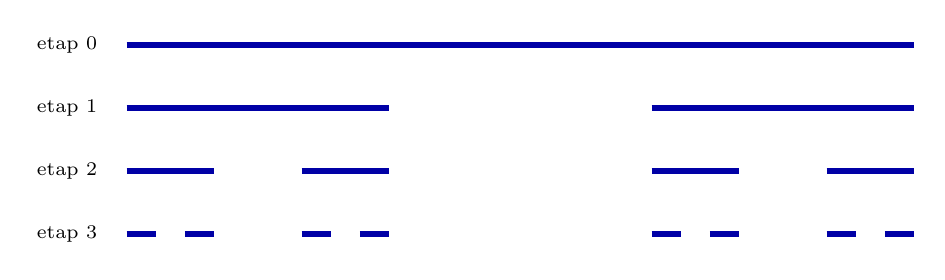
\begin{tikzpicture}[x=10cm,y=0.8cm]
\foreach \i/\y in {0/0,1/-1,2/-2,3/-3}{
 \ifnum\i=0
  \draw[line width=2pt,blue!65!black] (0,\y)--(1,\y);
 \fi
 \ifnum\i=1
  \draw[line width=2pt,blue!65!black] (0,\y)--(1/3,\y);
  \draw[line width=2pt,blue!65!black] (2/3,\y)--(1,\y);
 \fi
 \ifnum\i=2
  \foreach \a in {0,2/9,2/3,8/9}{\draw[line width=2pt,blue!65!black] (\a,\y)--({\a+1/9},\y);}
 \fi
 \ifnum\i=3
  \foreach \a in {0,2/27,2/9,8/27,2/3,20/27,8/9,26/27}{\draw[line width=2pt,blue!65!black] (\a,\y)--({\a+1/27},\y);}
 \fi
 \node[anchor=east,font=\scriptsize] at (-0.025,\y) {etap \i};
}
\end{tikzpicture}
\end{center}
\noindent\textit{Pierwsze etapy konstrukcji zbioru Cantora.}
Każde przejście zastępuje przedział dwoma
przedziałami o jednej trzeciej jego długości.

\begin{przyklad}[Gruby zbiór Cantora]
Zaczynamy od $F_0=[0,1]$. W kroku $n\ge1$
usuwamy ze środka każdego z $2^{n-1}$ pozostałych
przedziałów otwarty przedział długości $4^{-n}$.
Łączna długość usunięta do kroku $n$ wynosi
$\sum_{j=1}^n2^{j-1}4^{-j}=(1-2^{-n})/2$.
Wszystkie $2^n$ przedziały tworzące $F_n$ mają więc
długość $\ell_n=2^{-n-1}(1+2^{-n})$.
W szczególności $\ell_{n-1}>4^{-n}$, toteż każdy
krok jest wykonalny, a $\ell_n\to0$.
Zbiór $F=\bigcap_{n\ge0}F_n$ jest zwarty; z ciągłości
miary od góry otrzymujemy $\lambda_1(F)=1/2$.
Nie zawiera niepustego otwartego przedziału, ponieważ
taki przedział musiałby mieścić się w jednym przedziale
każdego poziomu $n$, a ich długości dążą do zera.
Zatem $F$ jest nigdzie gęsty. Na mocy twierdzenia~\ref{thm:euclidean-dimension-26}
ma wymiar Hausdorffa równy $1$, choć ma puste wnętrze.
Wymiar Hausdorffa nie charakteryzuje topologicznego
wymiaru ani posiadania wnętrza.
\end{przyklad}

\begin{wniosek}[Wykres funkcji Lipschitzowskiej]
\label{cor:graph-dimension-26}
Jeżeli $A\subseteq\mathbb R^m$ i
$f:A\to\mathbb R^k$ jest Lipschitzowska, to
$\dim_H\{(x,f(x)):x\in A\}=\dim_HA$.
\end{wniosek}
\begin{proof}
Odwzorowanie $x\mapsto(x,f(x))$ jest Lipschitzowskie,
więc nie zwiększa wymiaru Hausdorffa na mocy
twierdzenia~\ref{thm:hausdorff-lipschitz-26}.
Rzut $(x,y)\mapsto x$ jest również Lipschitzowski
i odwzorowuje wykres na $A$. Stosując tę samą
nierówność w drugą stronę, otrzymujemy równość.
\end{proof}

\section{Energie potencjałowe i wymiar}
\begin{definicja}[$t$-energia miary]
\label{def:energy-26}
Niech $t>0$, a $\mu$ będzie skończoną dodatnią miarą
borelowską na $\mathbb R^d$. Jej $t$-energią nazywamy
\[
 I_t(\mu)=\int_{\mathbb R^d}\!\int_{\mathbb R^d}
 |x-y|^{-t}\,\mathrm d\mu(y)\,\mathrm d\mu(x),
\]
przyjmując $|0|^{-t}=+\infty$. Całka należy do
$[0,+\infty]$; nie zakładamy jej skończoności.
\end{definicja}

\begin{twierdzenie}[Oszacowanie energii przez warunek Frostmana]
\label{thm:frostman-energy-26}
Jeżeli $\mu$ jest skończoną dodatnią miarą o
$\mu(B(x,r))\le Cr^s$ dla wszystkich $x,r$,
gdzie $s>0$, to $I_t(\mu)<\infty$ dla każdego
$0<t<s$.
\end{twierdzenie}
\begin{proof}
Z tożsamości warstwowej dla nieujemnych funkcji
$|x-y|^{-t}=t\int_{|x-y|}^{\infty}r^{-t-1}\,\mathrm dr$
i z twierdzenia Tonellego otrzymujemy
\[
 \int_{\mathbb R^d}|x-y|^{-t}\,\mathrm d\mu(y)
 =t\int_0^\infty r^{-t-1}\mu(B(x,r))\,\mathrm dr.
\]
W przedziale $(0,1)$ całka jest ograniczona przez
$Ct\int_0^1r^{s-t-1}\,\mathrm dr=Ct/(s-t)$.
W przedziale $(1,\infty)$ nie przekracza
$t\mu(\mathbb R^d)\int_1^\infty r^{-t-1}\,\mathrm dr
=\mu(\mathbb R^d)$. Oszacowanie jest jednostajne
względem $x$. Całkowanie po $x$ dowodzi tezy.
\end{proof}

\begin{twierdzenie}[Skończona energia a dolne oszacowanie wymiaru]
\label{thm:energy-dimension-26}
Niech $E\subseteq\mathbb R^d$ będzie zbiorem borelowskim,
$t>0$, a $\mu$ niezerową skończoną dodatnią miarą
borelowską skoncentrowaną na $E$. Jeśli $I_t(\mu)<\infty$,
to $\mathcal H^t(E)>0$, a zatem $\dim_HE\ge t$.
\end{twierdzenie}
\begin{proof}
Niech $U(x)=\int|x-y|^{-t}\,\mathrm d\mu(y)$.
Funkcja $U$ jest borelowska (jest półciągła z dołu
na mocy lematu Fatou) i $\int U\,\mathrm d\mu<\infty$,
więc $U$ jest skończona $\mu$-prawie wszędzie.
Istnieje liczba całkowita $M\ge1$ taka, że
$F=E\cap\{U\le M\}$ ma dodatnią $\mu$-miarę.
Kładziemy $\nu=\mu|_F$. Dla $z\in F$ i $r>0$
nierówność $|z-y|^{-t}\ge r^{-t}$ na $B(z,r)$
daje $\mu(B(z,r))\le Mr^t$.
Jeśli $B(x,r)\cap F=\varnothing$, to $\nu(B(x,r))=0$.
W przeciwnym przypadku wybieramy $z\in B(x,r)\cap F$,
a z inkluzji $B(x,r)\subseteq B(z,2r)$ otrzymujemy
$\nu(B(x,r))\le M2^tr^t$.
Zasada rozkładu masy~\ref{thm:mass-distribution-26}
zastosowana do $\nu$ na $F$ daje
$\mathcal H^t(E)\ge\mathcal H^t(F)>0$.
\end{proof}

\begin{wniosek}[Energetyczna charakteryzacja wymiaru zwartego zbioru]
\label{cor:energy-dimension-26}
Dla niepustego zwartego $K\subseteq\mathbb R^d$ zachodzi
\[
 \dim_H K=\sup\{t>0:\text{ istnieje miara probabilistyczna }
 \mu\text{ na }K,\ I_t(\mu)<\infty\},
\]
gdzie supremum pustego zbioru wynosi zero.
\end{wniosek}
\begin{proof}
Nierówność $\ge$ wynika z poprzedniego twierdzenia.
Jeżeli $0<t<\dim_H K$, wybieramy $s$ takie, że
$t<s<\dim_H K$. Wówczas $\mathcal H^s(K)=+\infty$,
więc twierdzenie Frostmana daje miarę probabilistyczną
na $K$ spełniającą warunek wzrostu masy kul z wykładnikiem
$s$. Twierdzenie~\ref{thm:frostman-energy-26}
zapewnia $I_t(\mu)<\infty$. Przechodzimy z $t$ do
$\dim_H K$ z dołu. Gdy $\dim_H K=0$, pierwsza
nierówność i konwencja o supremum kończą dowód.
\end{proof}

\begin{uwaga}[Dalsza perspektywa]
W rozdziałach dotyczących geometrycznej teorii miary
pojawią się miary prostowalne, wzór na pole powierzchni
i wzór koobszaru. Miara Hausdorffa nadaje im naturalną
skalę. Związek energii z pojemnością stanowi natomiast
punkt wyjścia do teorii potencjału, której pełne
rozwinięcie pozostawiamy do osobnego opracowania.
\end{uwaga}
